\documentclass[11pt, a4paper]{article}
\usepackage[utf8]{inputenc}
\usepackage{geometry}
\usepackage{xcolor}
\usepackage{hyperref}
\usepackage{graphicx}
\usepackage{amsmath}
\usepackage{algorithm}
\usepackage{algpseudocode}
\usepackage{tikz}
\usepackage{booktabs}
\usepackage{tcolorbox}
\usepackage{listings}
\usepackage{float}

\usetikzlibrary{shapes,arrows,positioning,shadows.blur,calc}
\geometry{margin=1in}

% --- Colors ---
\definecolor{swiftblue}{RGB}{0, 122, 255}
\definecolor{techdark}{RGB}{30, 30, 30}
\definecolor{successgreen}{RGB}{40, 167, 69}
\definecolor{warningorange}{RGB}{255, 193, 7}
\definecolor{codebg}{RGB}{245, 245, 245}

% --- Code Style ---
\lstdefinestyle{mystyle}{
    backgroundcolor=\color{codebg},   
    commentstyle=\color{green!50!black},
    keywordstyle=\color{blue},
    numberstyle=\tiny\color{gray},
    stringstyle=\color{red!70!black},
    basicstyle=\ttfamily\footnotesize,
    breakatwhitespace=false,         
    breaklines=true,                 
    captionpos=b,                    
    keepspaces=true,                 
    numbers=left,                    
    numbersep=5pt,                  
    showspaces=false,                
    showstringspaces=false,
    showtabs=false,                  
    tabsize=2,
    frame=single,
    rulecolor=\color{black!10}
}
\lstset{style=mystyle}

\lstdefinelanguage{JavaScript}{
  keywords={break, case, catch, class, const, continue, debugger, default, delete, do, else, enum, export, extends, false, finally, for, function, if, import, in, instanceof, new, null, return, super, switch, this, throw, true, try, typeof, var, void, while, with, let, async, await, yield},
  keywordstyle=\color{blue}\bfseries,
  ndkeywords={class, export, boolean, throw, implements, import, this},
  ndkeywordstyle=\color{techdark}\bfseries,
  identifierstyle=\color{black},
  sensitive=false,
  comment=[l]{//},
  morecomment=[s]{/*}{*/},
  commentstyle=\color{green!50!black}\ttfamily,
  stringstyle=\color{red!70!black}\ttfamily,
  morestring=[b]',
  morestring=[b]"
}

\lstdefinelanguage{TypeScript}{
  keywords={abstract, any, as, boolean, break, case, catch, class, console, const, continue, debugger, declare, default, delete, do, else, enum, export, extends, false, finally, for, from, function, get, if, implements, import, in, infer, instanceof, interface, is, keyof, let, module, namespace, never, new, null, number, object, package, private, protected, public, readonly, require, return, set, static, string, super, switch, symbol, this, throw, true, try, type, typeof, undefined, unique, unknown, var, void, while, with, yield, async, await},
  keywordstyle=\color{blue}\bfseries,
  ndkeywords={class, export, boolean, throw, implements, import, this},
  ndkeywordstyle=\color{techdark}\bfseries,
  identifierstyle=\color{black},
  sensitive=true,
  comment=[l]{//},
  morecomment=[s]{/*}{*/},
  commentstyle=\color{green!50!black}\ttfamily,
  stringstyle=\color{red!70!black}\ttfamily,
  morestring=[b]',
  morestring=[b]"
}

\title{\textbf{\Huge SwiftJS Architecture v0.7}\\ \Large Deep Dive: Algorithms \& Optimizations}
\author{SwiftJS Core Team}
\date{\today}

\begin{document}

\maketitle

% --- Executive Summary ---
\begin{tcolorbox}[colback=swiftblue!5,colframe=swiftblue,title=\textbf{Executive Summary}]
SwiftJS v0.7.0 achieves \textbf{53,215 req/sec} by fundamentally re-engineering the Node.js request lifecycle. This whitepaper details the specific algorithms (Iterative Radix Tree, Hybrid Execution) and memory techniques (Lazy Parsing, Context Pooling) that eliminate the "framework tax" found in Express/NestJS.
\end{tcolorbox}

\tableofcontents

\section{1. The Hybrid Execution Engine}

\subsection{Problem: The Async Tax}
In standard Node.js frameworks (e.g., Koa, Express v5), the entire middleware chain is wrapped in Promises. Even a simple synchronous "Health Check" endpoint pays the cost of:
\begin{itemize}
    \item Promise allocation per middleware.
    \item Microtask queue scheduling (Next Tick).
    \item Context switching overhead.
\end{itemize}

\subsection{Solution: Dual-Mode Router}
SwiftJS implements a router that inspects the handler's return type. If the handler is synchronous, it executes immediately on the stack.

\begin{algorithm}[H]
\caption{Hybrid Execution Flow}\label{alg:hybrid}
\begin{algorithmic}[1]
\Function{HandleRequest}{ctx}
    \State $route \gets \Call{Lookup}{ctx.path}$
    \If{$route.isSync$ \textbf{and} \textbf{not} $hasAsyncMiddleware$}
        \State \Comment{\textbf{Fast Path}: Zero Allocation}
        \State \Call{route.handler}{ctx} 
        \State \Return
    \EndIf
    \State \Comment{\textbf{Slow Path}: Promise Wrappers}
    \State \Return \Call{ExecuteAsyncPipeline}{ctx, route}
\EndFunction
\end{algorithmic}
\end{algorithm}

\subsubsection{Before vs. After Comparison}

\begin{minipage}{0.48\textwidth}
\textbf{Before (Standard Approach)}
\begin{lstlisting}[language=JavaScript]
async function handle(req, res) {
  // Always returns a Promise
  await middleware1(ctx);
  await middleware2(ctx);
  await handler(ctx); 
}
\end{lstlisting}
\end{minipage}
\hfill
\begin{minipage}{0.48\textwidth}
\textbf{After (SwiftJS Optimization)}
\begin{lstlisting}[language=TypeScript]
function handle(ctx): void | Promise<void> {
  // Returns void if sync
  if (isSync) {
    middleware1(ctx);
    handler(ctx);
    return; 
  }
  // Allocates only if needed
  return runAsync(ctx);
}
\end{lstlisting}
\end{minipage}

\subsection{File-System Routing Engine}
SwiftJS employs a \textbf{convention-over-configuration} file router that maps the directory structure directly to URL paths. Unlike naive implementations that scan sequentially, SwiftJS uses a parallelized loading strategy.

\begin{algorithm}[H]
\caption{Parallel Route Loading}\label{alg:fs-routing}
\begin{algorithmic}[1]
\Function{LoadRoutes}{dir}
    \State $files \gets \Call{ScanRecursive}{dir}$
    \State $promises \gets []$
    \ForAll{$file \in files$}
        \If{$file$ matches `.*\.(method)\.(ts|js)`}
            \State $promises.push(\Call{ImportModule}{file})$
        \EndIf
    \EndFor
    \State \Comment{Parallel V8 Compile \& Execute}
    \State $modules \gets \textbf{await} \textbf{Promise}.all(promises)$
    \State \Return $modules.map(m \to \Call{Register}{m})$
\EndFunction
\end{algorithmic}
\end{algorithm}

\begin{figure}[H]
\centering
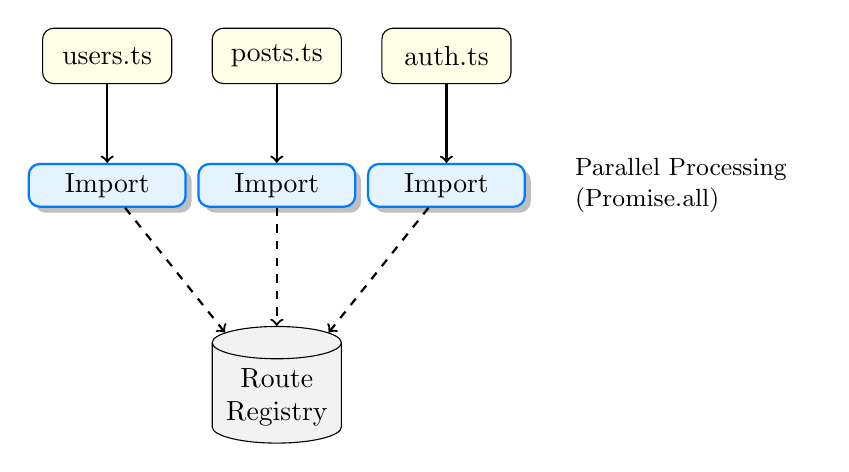
\begin{tikzpicture}[node distance=1.5cm, auto,
    file/.style={rectangle, draw=black, fill=yellow!10, thin, minimum height=2em, text width=4em, text centered, rounded corners},
    process/.style={rectangle, draw=swiftblue, fill=swiftblue!10, thick, text width=5em, text centered, rounded corners, drop shadow},
    registry/.style={cylinder, shape border rotate=90, draw=black, fill=gray!10, aspect=0.25, text width=4em, text centered}
]

    \node[file] (f1) {users.ts};
    \node[file, right=0.5cm of f1] (f2) {posts.ts};
    \node[file, right=0.5cm of f2] (f3) {auth.ts};
    
    \node[process, below=1cm of f1] (p1) {Import};
    \node[process, below=1cm of f2] (p2) {Import};
    \node[process, below=1cm of f3] (p3) {Import};
    
    \node[registry, below=1.5cm of p2] (reg) {Route Registry};

    \draw[->, thick] (f1) -- (p1);
    \draw[->, thick] (f2) -- (p2);
    \draw[->, thick] (f3) -- (p3);
    
    \draw[->, thick, dashed] (p1) -- (reg);
    \draw[->, thick, dashed] (p2) -- (reg);
    \draw[->, thick, dashed] (p3) -- (reg);
    
    \node[right=0.5cm of p3, text width=3cm, font=\small] {Parallel Processing (Promise.all)};

\end{tikzpicture}
\caption{Parallel Module Loading Pipeline}
\end{figure}

\subsubsection{Path Mapping conventions}
\begin{itemize}
    \item \textbf{Static:} `routes/users/list.get.ts` $\rightarrow$ `GET /users/list`
    \item \textbf{Dynamic:} `routes/users/[id].get.ts` $\rightarrow$ `GET /users/:id`
    \item \textbf{Mixed:} `routes/posts/[postId]/comments.get.ts` $\rightarrow$ `GET /posts/:postId/comments`
\end{itemize}

\begin{figure}[H]
\centering
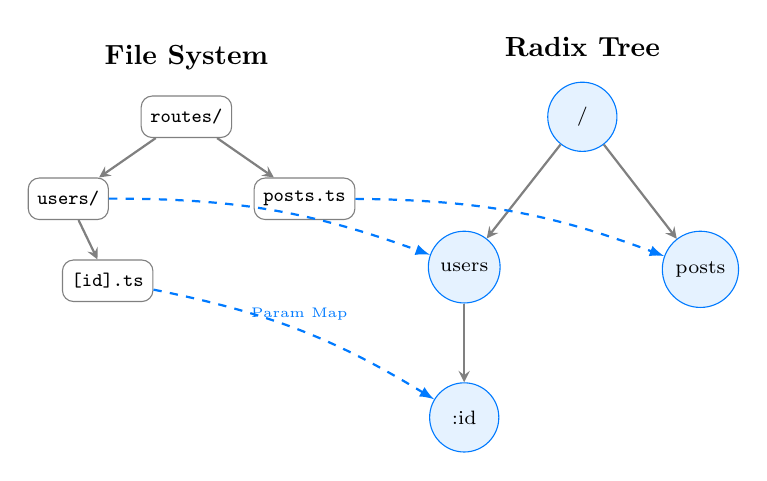
\begin{tikzpicture}[
    fsnode/.style={rectangle, draw=gray, fill=white, rounded corners, minimum height=1.5em, font=\ttfamily\scriptsize},
    trienode/.style={circle, draw=swiftblue, fill=swiftblue!10, minimum size=2.5em, font=\scriptsize, align=center},
    edge/.style={->, >=stealth, thick, gray},
    map/.style={->, >=latex, dashed, thick, swiftblue}
]

    % File System Tree
    \node[fsnode] (root) {routes/};
    \node[fsnode, below=0.5cm of root, xshift=-1.5cm] (users) {users/};
    \node[fsnode, below=0.5cm of users, xshift=0.5cm] (uid) {[id].ts};
    \node[fsnode, below=0.5cm of root, xshift=1.5cm] (posts) {posts.ts};

    \draw[edge] (root) -- (users);
    \draw[edge] (users) -- (uid);
    \draw[edge] (root) -- (posts);

    % Radix Tree
    \node[trienode, right=4cm of root] (troot) {/};
    \node[trienode, below=1cm of troot, xshift=-1.5cm] (tusers) {users};
    \node[trienode, below=1cm of tusers] (tuid) {:id};
    \node[trienode, below=1cm of troot, xshift=1.5cm] (tposts) {posts};

    \draw[edge] (troot) -- (tusers);
    \draw[edge] (tusers) -- (tuid);
    \draw[edge] (troot) -- (tposts);

    % Mapping arrows
    \draw[map] (users) to[bend left=10] (tusers);
    \draw[map] (uid) to[bend left=10] node[midway, above, font=\tiny\color{swiftblue}] {Param Map} (tuid);
    \draw[map] (posts) to[bend left=10] (tposts);

    \node[above=0.2cm of root, font=\bfseries] {File System};
    \node[above=0.2cm of troot, font=\bfseries] {Radix Tree};

\end{tikzpicture}
\caption{Structural Mapping: Directory Layout $\to$ Routing Trie}
\end{figure}

\section{2. Zero-Allocation Routing}

\subsection{Radix Tree Architecture}
We use a specialized \textbf{Compact Prefix Tree (Radix Tree)} optimized for HTTP paths. Key features:
\begin{itemize}
    \item \textbf{Param Separation:} Static nodes are checked first ($O(1)$ Hash Map lookup). Parameter nodes (`/:id`) are checked only on miss.
    \item \textbf{Iterative Backtracking:} Replaces recursion with a `while` loop to prevent stack overflow and reduce function call overhead.
\end{itemize}

\begin{algorithm}[H]
\caption{Iterative Radix Lookup (Optimized)}\label{alg:radix}
\begin{algorithmic}[1]
\Function{FindRoute}{method, path}
    \State $node \gets root$, $i \gets 0$, $stack \gets []$
    \While{$node \neq \text{null}$}
        \If{$i = length(segments)$}
            \If{$node.handlers[method]$} \Return $match$ \EndIf
            \State \textbf{Backtrack:} $state \gets stack.pop()$
            \State $node \gets state.node$, $i \gets state.i$
            \State \textbf{continue}
        \EndIf
        
        \State $segment \gets segments[i]$
        \State \Comment{Prioritize Static Match (O(1))}
        \If{$node.staticChildren.has(segment)$}
            \State $stack.push(\{node, i, \text{tryParam: true}\})$
            \State $node \gets node.staticChildren.get(segment)$
            \State $i \gets i + 1$
            \State \textbf{continue}
        \EndIf
        
        \State \Comment{Fallback to Param/Wildcard}
        \If{$node.paramChild$}
            \State $params[name] \gets segment$
            \State $node \gets node.paramChild$
            \State $i \gets i + 1$
        \Else
            \State \textbf{Backtrack}
        \EndIf
    \EndWhile
\EndFunction
\end{algorithmic}
\end{algorithm}

\section{3. Memory \& Context Optimization}

\subsection{Object Pooling}
To keep Garbage Collection (GC) pauses under 5ms (critical for real-time apps), SwiftJS reuses the central `HttpContext` object.

\begin{lstlisting}[language=TypeScript]
const pool: HttpContext[] = [];

// acquire() - O(1)
function getContext(req, res) {
  if (pool.length > 0) {
    const ctx = pool.pop();
    ctx.reset(req, res); // Reset specific props only
    return ctx;
  }
  return new HttpContext(req, res);
}

// release() - O(1)
function releaseContext(ctx) {
  if (pool.length < MAX_SIZE) {
    pool.push(ctx);
  }
}
\end{lstlisting}

\subsection{Lazy Evaluation Strategy}
Parsing everything upfront (Express/Connect style) wastes CPU on unused data. SwiftJS parses lazily:

\begin{itemize}
    \item \textbf{Query String:} `ctx.query` uses a getter. If the handler doesn't access it, the URL parser never runs.
    \item \textbf{Cookies:} `ctx.cookies` parses the raw `Cookie` header only on first access.
    \item \textbf{Body:} `ctx.body` is not parsed automatically for GET/HEAD requests.
\end{itemize}

\section{4. Pre-Computed Response Headers}

\subsection{Technique}
Creating new objects like `{ 'Content-Type': 'application/json' }` for every response triggers allocation. SwiftJS uses shared constants.

\begin{lstlisting}[language=TypeScript]
const JSON_HEADERS = { 'Content-Type': 'application/json' };

// SwiftJS Implementation
class Response {
  json(data) {
    if (!this.headersSent) {
      // Zero-allocation: pass reference to existing object
      this.writeHead(200, JSON_HEADERS); 
    }
    this.end(JSON.stringify(data));
  }
}
\end{lstlisting}

\section{Summary of Optimizations}

\begin{table}[h]
\centering
\begin{tabular}{@{} l l l @{}}
\toprule
\textbf{Technique} & \textbf{Traditional Impact} & \textbf{SwiftJS Optimization} \\
\midrule
Routing & Recursive, Dynamic (RegExp) & \textbf{Iterative Radix Tree} \\
Async & Promise.all / Await Chain & \textbf{Hybrid Sync/Async} \\
Memory & New Context per Request & \textbf{Context Pooling} \\
Parsing & Eager (Upfront) & \textbf{Lazy (On-Demand)} \\
Headers & Dynamic Allocation & \textbf{Static Constants} \\
\bottomrule
\end{tabular}
\caption{Architectural Improvements Overview}
\end{table}

\end{document}
